\chapter{Assembly}
\section{Linguaggi di alto e basso livello}
\subsection{Linguaggio assembler}
\subsubsection{Cosa è?}
È una rappresentazione simbolica del linguaggio macchina rendendolo così molto più comprensibile.

Viene tradotto dall'assemblatore in linguaggio macchina

\subsubsection{Vantaggi}
La dipendenza dall'architettura del calcolatore permette:
\begin{itemize}
    \item Ottimizzare le prestazioni (maggiore efficienza)
    \item Programmi (potenzialmente) più compatti
    \item Massimo sfruttamento delle potenzialità dell'hardware sottostante
    \item Molto importante per programmare controller di processi  e macchinari, o per apparati limitati
\end{itemize}

\subsubsection{Svantaggi}

\begin{itemize}
    \item Minore espressività
    \item Necessario conoscere i dettagli dell'architettura
    \item Mancanza di portabilità su architetture diverse
    \item Difficoltà di comprensione
    \item Lunghezza maggiore dei programmi
\end{itemize}

\subsection{Linguaggi ad alto livello}
\subsubsection{Cosa sono?}
Sono linguaggi facilmente utilizzabili per gli umani, vengono compilati (o interpretati) per poi essere tradotti in assembler

\subsubsection{Vantaggi}
\begin{itemize}
    \item Notazione vicina al linguaggio corrente e alta notazione algebrica (maggiore espressività e leggibilità)
    \item Incremento della produttività, la programmazione è svincolata dala conoscenza dei dettagli architetturali della macchina utilizzata
    \item Indipendenza dalle caratteristiche dell'architettura su cui il programma va eseguito
    \item Permettono l'uso di librerie di funzionalità dià scritte
\end{itemize}

\section{Catena programmativa (Vista ad alto livello)}
\subsection{Struttura}
\begin{center}
    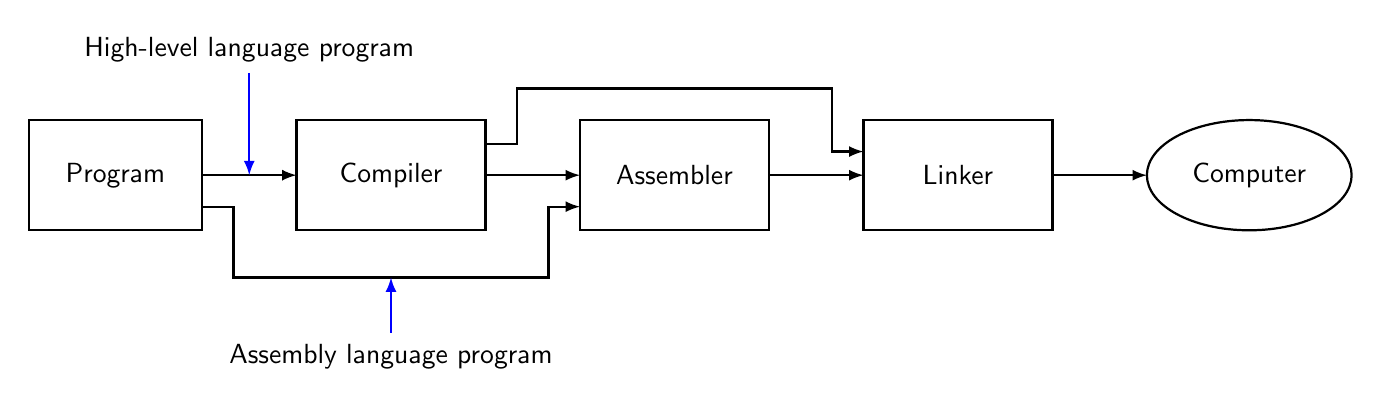
\begin{tikzpicture}[thick, >=latex, font=\sffamily]

        % 1. Blocchi rettangolari
        \draw (0, 0) rectangle (2.2, 1.4);
        \node at (1.1, 0.7) {Program};

        \draw (3.4, 0) rectangle (5.8, 1.4);
        \node at (4.6, 0.7) {Compiler};

        \draw (7.0, 0) rectangle (9.4, 1.4);
        \node at (8.2, 0.7) {Assembler};

        \draw (10.6, 0) rectangle (13.0, 1.4);
        \node at (11.8, 0.7) {Linker};

        % 2. Blocco Computer (rettangolo con angoli arrotondati o ellisse standard)
        \draw (15.5, 0.7) ellipse (1.3cm and 0.7cm);
        \node at (15.5, 0.7) {Computer};

        % 3. Frecce orizzontali principali
        \draw[->] (2.2, 0.7) -- (3.4, 0.7);
        \draw[->] (5.8, 0.7) -- (7.0, 0.7);
        \draw[->] (9.4, 0.7) -- (10.6, 0.7);
        \draw[->] (13.0, 0.7) -- (14.2, 0.7);

        % 4. Freccia e testo in alto (High-level language program)
        \node[align=center] at (2.8, 2.3) {High-level language program};
        \draw[->, blue] (2.8, 2.0) -- (2.8, 0.7);

        % 5. Bypass inferiore per Assembly (Program -> Assembler)
        \draw[->] (2.2, 0.3) -- (2.6, 0.3) -- (2.6, -0.6) -- (6.6, -0.6) -- (6.6, 0.3) -- (7.0, 0.3);

        % 6. Freccia e testo in basso (Assembly language program)
        \node[align=center] at (4.6, -1.6) {Assembly language program};
        \draw[->, blue] (4.6, -1.3) -- (4.6, -0.6);

        % 7. Bypass superiore per Compiler -> Linker
        \draw[->] (5.8, 1.1) -- (6.2, 1.1) -- (6.2, 1.8) -- (10.2, 1.8) -- (10.2, 1.0) -- (10.6, 1.0);

    \end{tikzpicture}
\end{center}

\subsection{Ruolo del Compiler}
\begin{itemize}
    \item Un programma ad alto livello viene tradotto nel linguaggio assembler utilizzando un apposito programma: il compilatore.
    
    \item Dopo la fase di compilazione, il programma scritto in linguaggio assembler viene tradotto in linguaggio macchina da un apposito programma: l'assemblatore
\end{itemize}

\section{Catena programmativa (Vista a basso livello)}
\subsection{Struttura}
\begin{center}
    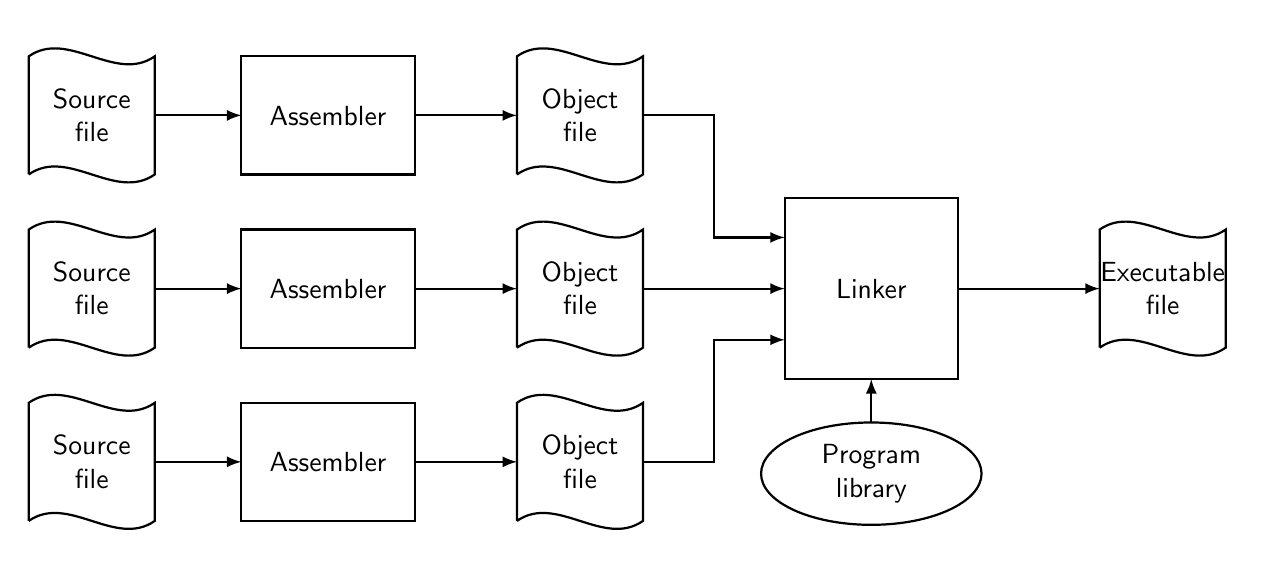
\begin{tikzpicture}[thick, >=latex, font=\sffamily]

        % --- Fogli ondulati (Source, Object, Executable) ---
        \foreach \x/\y/\tA/\tB in {
            0/4.4/Source/file,
            0/2.2/Source/file,
            0/0/Source/file,
            6.2/4.4/Object/file,
            6.2/2.2/Object/file,
            6.2/0/Object/file,
            13.6/2.2/Executable/file
        } {
            \draw (\x, \y) -- (\x, \y+1.5)
                .. controls (\x+0.5, \y+1.85) and (\x+1.1, \y+1.15) .. (\x+1.6, \y+1.5)
                -- (\x+1.6, \y)
                .. controls (\x+1.1, \y-0.35) and (\x+0.5, \y+0.35) .. (\x, \y);
            \node[align=center] at (\x+0.8, \y+0.75) {\tA\\\tB};
        }

        % --- Blocchi Assembler ---
        \foreach \y in {4.4, 2.2, 0} {
            \draw (2.7, \y) rectangle (4.9, \y+1.5);
            \node at (3.8, \y+0.75) {Assembler};
            % Frecce Source -> Assembler -> Object
            \draw[->] (1.6, \y+0.75) -- (2.7, \y+0.75);
            \draw[->] (4.9, \y+0.75) -- (6.2, \y+0.75);
        }

        % --- Blocco Linker (altezza aumentata per raccogliere bene le 3 frecce) ---
        \draw (9.6, 1.8) rectangle (11.8, 4.1);
        \node at (10.7, 2.95) {Linker};

        % --- Frecce Object files -> Linker ---
        % Superiore
        \draw[->] (7.8, 5.15) -- (8.7, 5.15) -- (8.7, 3.6) -- (9.6, 3.6);
        % Centrale (perfettamente orizzontale)
        \draw[->] (7.8, 2.95) -- (9.6, 2.95);
        % Inferiore
        \draw[->] (7.8, 0.75) -- (8.7, 0.75) -- (8.7, 2.3) -- (9.6, 2.3);

        % --- Program library (ellisse) e freccia verso il Linker ---
        \draw (10.7, 0.6) ellipse (1.4cm and 0.65cm);
        \node[align=center] at (10.7, 0.6) {Program\\library};
        \draw[->] (10.7, 1.25) -- (10.7, 1.8);

        % --- Freccia Linker -> Executable file (perfettamente orizzontale sull'asse centrale) ---
        \draw[->] (11.8, 2.95) -- (13.6, 2.95);

    \end{tikzpicture}
\end{center}

\newpage
\subsection{Assembler}
\subsubsection{Cosa fa?}
\begin{itemize}
    \item Converte un programma assembler (file sorgente) in linguaggio macchina (file oggetto)
    \item Gestisce le etichette
    \item Gestisce le pseudoistruzioni
    \item Gestisce numeri in base diverse
\end{itemize}

\subsubsection{Processo di assemblaggio}
L'assemblaggio è un procedimento sequenziale che esamini, riga per riga, il codice sorgente Assembly, traducendo ciascuna riga in un'istruzione del linguaggio macchina. 

Questo processo di assemblaggio viene applicato modulo per modulo al programma e costituisce per ogni modulo la tabella dei simboli del modulo, questo avviene in 2 passaggi principali:

\begin{enumerate}
    \item Traduce i codici mnemonici (\texttt{add, addi, sub, lw, sw, j, etc etc}) delle istruzioni nei corrispondenti codici binari
    \item Traduce i riferimenti simbolici (variabili, registri, etichette di salto, parametri) nei corrispondenti indirizzi numerici
\end{enumerate}

Ogni lettura del programma sorgente è chiamata passo e l'assemblatore è chiamato traduttore a due passi, ogni modulo assemblato di default parte dall'indirizzo 0, in sistemi dotatti di meccanismi di memoria virtuale tali indirizzi sono indirizzi virtuali

\subsubsection{Tabella dei Simboli}
La tabella dei simboli contiene i riferimenti simbolici presenti nel modulo da tradurre e, al termine del primo passo, conterrà gli indirizzi numerici di tutti i simboli, tranne quelli esterni al modulo in esame.

Per le etichette associate a direttive dell'assemblatore che definiscono costanti simboliche nella tabella dei simboli viene creata la coppia \texttt{<etichetta, valore>} e in ogni istruzione che fa riferimento al simbolo viene sostituito il valore.

Per etichette  che definiscono variabili (spazio di memoria + eventuale inizializzazione), l'assemblatore riserva spazio, eventualmente inizializza la zona di memoria e crea nella tabella la coppia \texttt{<etichetta, indirizzo>}. In ogni istruzione che fa riferimento al simbolo viene sostituito l'indirizzo.

Nelle etichette presenti nelle istruzioni di salto, l'assemblatore deve generare un riferimento all'indirizzo dell'istruzione destinazione di salto

\newpage
\subsection{Linker (Link editor)}
\subsubsection{Cosa fa?}
\begin{itemize}
    \item Inserisce in memoria in modo simbolico il codice e i moduli dati
    \item Determina gli indirizzi dei dati e delle etichette che compaiono nelle istruzioni
    \item Corregge i riferimenti interni ed esterni e risolve i riferimenti in sospeso (a etichette esterne)
    \item Genera il file eseguibile
    \item Lettura dell'intestazione del file eseguibile per determinare la lunghezza del segmento di testo e del segmento dati
    \item Creazione di uno spazio di indirezzamento sufficiente a contenere testo e dati
    \item Copia delle istruzioni e dati dal file eseguibile in memoria
    \item Copia nello stack degli eventuali parametri passati al programma principale
    \item Inizializzazione dei registri e impostazione dello stack pointer affinchè punti alla prima locazione libera
    \item Salto a una procedura di startup la quale copia i parametri nei registri argomento e chiama la procedura principale del programma
    \item Quando la procedura principale restituisce il controllo, la procedura di startup termina il programma con una chiamata alla funzione di sistema exit
\end{itemize}
\subsubsection{Strttura}
\begin{center}
    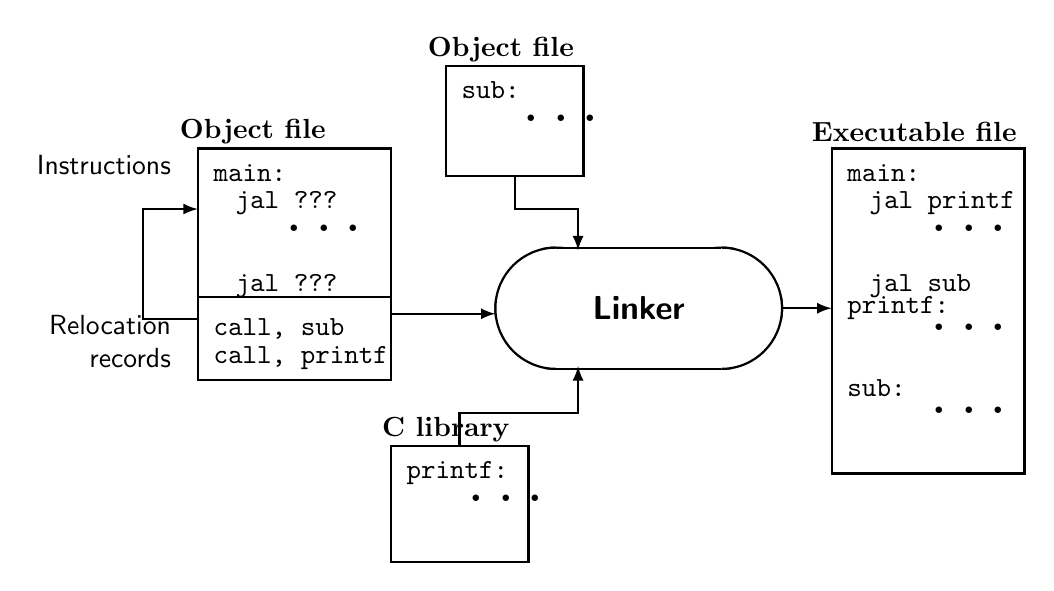
\begin{tikzpicture}[thick, >=latex, font=\sffamily, scale=0.7]

        % ==========================================
        % 1. BLOCCO CENTRALE: LINKER (Stadio ellittico)
        % ==========================================
        \draw (8.0, 3.0) rectangle (11.0, 5.2);
        \draw (8.0, 4.1) circle [x radius=1.1, y radius=1.1];
        \draw (11.0, 4.1) circle [x radius=1.1, y radius=1.1];
        % Ridisegno i bordi orizzontali puliti del "pill" shape
        \fill[white] (6.9, 3.0) rectangle (12.1, 5.2);
        \draw (8.0, 5.2) -- (11.0, 5.2);
        \draw (8.0, 3.0) -- (11.0, 3.0);
        \draw (8.0, 5.2) arc[start angle=90, end angle=270, radius=1.1];
        \draw (11.0, 3.0) arc[start angle=-90, end angle=90, radius=1.1];
        \node[font=\sffamily\bfseries\large] at (9.5, 4.1) {Linker};

        % ==========================================
        % 2. BLOCCO SINISTRO: OBJECT FILE PRINCIPALE
        % ==========================================
        \node[font=\bfseries] at (2.5, 7.3) {Object file};
        
        % Riquadro Istruzioni (superiore)
        \draw (1.5, 4.3) rectangle (5.0, 7.0);
        \node[anchor=north west, font=\ttfamily] at (1.6, 6.9) {main:};
        \node[anchor=north west, font=\ttfamily] at (2.0, 6.4) {jal ???};
        \node[anchor=north west, font=\ttfamily] at (2.8, 5.8) {\huge \textbf{\dots}};
        \node[anchor=north west, font=\ttfamily] at (2.0, 4.9) {jal ???};

        % Riquadro Relocation records (inferiore)
        \draw (1.5, 2.8) rectangle (5.0, 4.3);
        \node[anchor=north west, font=\ttfamily] at (1.6, 4.1) {call, sub};
        \node[anchor=north west, font=\ttfamily] at (1.6, 3.6) {call, printf};

        % Etichette a sinistra e freccia di richiamo relocation
        \node[align=right, anchor=east] at (1.2, 6.7) {Instructions};
        \node[align=right, anchor=east] at (1.2, 3.5) {Relocation\\records};
        \draw[->] (1.5, 3.9) -- (0.5, 3.9) -- (0.5, 5.9) -- (1.5, 5.9);

        % Freccia Object file -> Linker
        \draw[->] (5.0, 4.0) -- (6.9, 4.0);

        % ==========================================
        % 3. BLOCCO SUPERIORE: OBJECT FILE (sub)
        % ==========================================
        \node[font=\bfseries] at (7.0, 8.8) {Object file};
        \draw (6.0, 6.5) rectangle (8.5, 8.5);
        \node[anchor=north west, font=\ttfamily] at (6.1, 8.4) {sub:};
        \node[anchor=north west, font=\ttfamily] at (7.1, 7.8) {\huge \textbf{\dots}};

        % Freccia a gomito verso il Linker
        \draw[->] (7.25, 6.5) -- (7.25, 5.9) -- (8.4, 5.9) -- (8.4, 5.15);

        % ==========================================
        % 4. BLOCCO INFERIORE: C LIBRARY
        % ==========================================
        \node[font=\bfseries] at (6.0, 1.9) {C library};
        \draw (5.0, -0.5) rectangle (7.5, 1.6);
        \node[anchor=north west, font=\ttfamily] at (5.1, 1.5) {printf:};
        \node[anchor=north west, font=\ttfamily] at (6.1, 0.9) {\huge \textbf{\dots}};

        % Freccia a gomito verso il Linker
        \draw[->] (6.25, 1.6) -- (6.25, 2.2) -- (8.4, 2.2) -- (8.4, 3.05);

        % ==========================================
        % 5. BLOCCO DESTRO: EXECUTABLE FILE
        % ==========================================
        \node[font=\bfseries] at (14.5, 7.3) {Executable file};
        \draw (13.0, 1.1) rectangle (16.5, 7.0);

        \node[anchor=north west, font=\ttfamily] at (13.1, 6.9) {main:};
        \node[anchor=north west, font=\ttfamily] at (13.5, 6.4) {jal printf};
        \node[anchor=north west, font=\ttfamily] at (14.5, 5.8) {\huge \textbf{\dots}};
        \node[anchor=north west, font=\ttfamily] at (13.5, 4.9) {jal sub};

        \node[anchor=north west, font=\ttfamily] at (13.1, 4.5) {printf:};
        \node[anchor=north west, font=\ttfamily] at (14.5, 4.0) {\huge \textbf{\dots}};

        \node[anchor=north west, font=\ttfamily] at (13.1, 3.0) {sub:};
        \node[anchor=north west, font=\ttfamily] at (14.5, 2.5) {\huge \textbf{\dots}};

        % Freccia Linker -> Executable file
        \draw[->] (12.1, 4.1) -- (13.0, 4.1);

    \end{tikzpicture}
\end{center}

\newpage
\section{Convenzioni nomi ed uso dei registri}

\begin{center}
    \begin{tabular}{ |c|c|c| }
        \hline
        \textbf{Nome simbolico} & \textbf{Numero} & \textbf{Uso} \\
        \hline
        \$zero & 0 & Costante 0 \\ 
        \hline
        \$at & 1 & \textcolor{red}{"Variabile" temporanea dell'assembler} \\
        \hline
        \$v0-\$v1 & 2-3 & \textcolor{red}{Valutazione di funzioni ed espressioni} \\
        \hline
        \$a0-\$a3 & 4-7 & \textcolor{red}{Argomento di "funzione"}\\
        \hline
        \$t0-\$t7 & 8-15 & \textcolor{blue}{"Variabili" temporanee} \\
        \hline
        \$s0-\$s7 & 16-23 & \textcolor{red}{Variabili} \textcolor{blue}{temporanee} \textcolor{red}{salvate} \\
        \hline
        \$t8-\$t9 & 8-15 & \textcolor{blue}{"Variabili" temporanee} \\
        \hline
        \$k0- \$k1 & 26-27 & \textcolor{red}{Riservati per il kernel del SO} \\
        \hline
        \$gp & 28 & \textcolor{red}{Global pointer} \\
        \hline
        \$sp & 29 & \textcolor{red}{Stack pointer} \\
        \hline
        \$fp & 30 & \textcolor{red}{Frame pointer} \\
        \hline
        \$ra & 31 & \textcolor{red}{Return address} \\
        \hline
    \end{tabular}

    \begin{itemize}
        \item \textcolor{red}{Usati da assembler, compilatore, sistema operativo}
        \item Secondo specifiche \textcolor{red}{convenzioni}
    \end{itemize}
\end{center}

\section{Direttive all'assemblatore}
\subsection{Cosa sono?}
Sono indicazioni date all'assembler per consentirgli di:
\begin{itemize}
    \item Associare etichette simboliche a indirizzi
    \item Allocare spazio di memoria per le variabili
    \item Decidere in quali zone di memoria allocare istruzioni e dati
    \item ...
\end{itemize}

\subsection{Esempi di direttive}
\begin{itemize}
    \item \texttt{.data <addr>}
    \begin{itemize}
        \item Quel che segue va nel segmento dati (eventualmente dall'indirizzo addr)
    \end{itemize}

    \item \texttt{.byte $b_1,\dots,b_n$}
    \begin{itemize}
        \item Inizializza i valori in byte successivi
    \end{itemize}

    \item \texttt{.word $w_1,\dots,w_n$}
    \begin{itemize}
        \item Inizializza i valori in word successive
    \end{itemize}

    \item \texttt{.text <addr>}
    \begin{itemize}
        \item Quel che segue va nel segmento text(programma) (eventualmente dall'indirizzo addr)
    \end{itemize}
\end{itemize}

\newpage
\subsection{Esempio d'uso}
\begin{lstlisting}
item:
    .data
    .word1
    .text
    .globl main

main:
    la $t0, item    #carico l'indirizzo di memoria della variabile item in $t0
    lw $t1, 0($t0)  #carico in $t1 il valore che si trova all'indirizzo 
                    #all'indirizzo di memoria 0 piu' il valore che sta nel registro $t0
\end{lstlisting}

\section{Pseudoistruzioni}
\subsection{Cosa sono?}
Sono istruzioni assembly che non hanno una corrispondete istruzione macchina, per far si che il programma funzioni vengono tradotte dall'assembler in una sequenza di istruzioni

\subsection{Esempio 1}
\begin{itemize}
    \item \texttt{li rdest, imm}
    \begin{itemize}
        \item load immediate
        \item Carica una costante di 32 bit nel registro rdest
    \end{itemize}
\end{itemize}
\begin{center}
    \texttt{li \$s0, 4000000}
\end{center}

\subsection{Esempio 2}
\begin{itemize}
    \item \texttt{move \$t0, \$t1}
    \begin{itemize}
        \item Tradotta dall'assemblatore in \texttt{add \$t0, \$zero, \$t1}
    \end{itemize}
\end{itemize}

\section{Flusso di controllo}
\subsection{Problema}
\begin{center}
    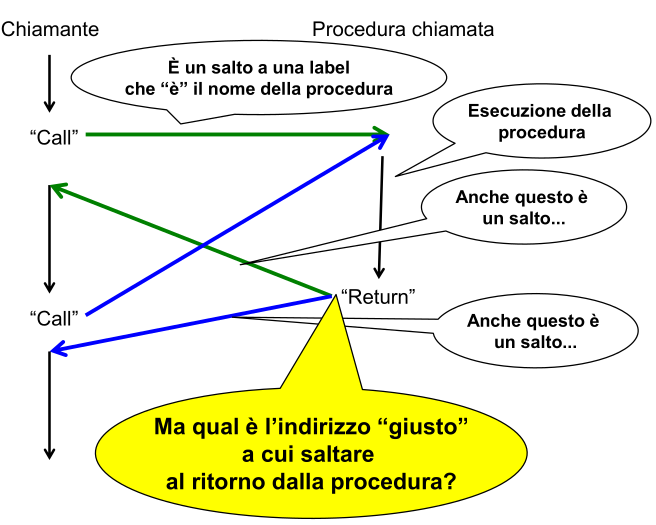
\includegraphics[scale=0.46]{Immagini/Flusso di controllo.png}
\end{center}

\subsection{Istruzione jal - Jump And Link}
\subsubsection{Cosa fa?}
\begin{itemize}
    \item Salta a una procedura indicata nell'istruzione e contemporaneamente  crea un collegamento a dove deve ritornare per continuare l'esecuzione del chiamante
    
    \item Salva nel registro \$ra l'indirizzo a cui tornare dopo l'esecuzione della procedura
\end{itemize}

\subsubsection{Esempio in assembly}
\begin{lstlisting}
.data
    risultato: .word 0

.text
.globl main

main:
    li   $a0, 5                # Parametro di input: $a0 = 5
    jal  raddoppia             # Chiamata a procedura: salta a 'raddoppia' e salva PC+4 in $ra
    
rientro_main:                 # <-- $ra puntera' all'indirizzo di questa istruzione!
    sw   $v0, risultato        # Salva il risultato restituito ($v0) in memoria
    
    # Chiusura del programma
    li   $v0, 10               
    syscall

# ----------------------------------------------------
# Procedura foglia 'raddoppia': calcola $v0 = $a0 * 2
# ----------------------------------------------------
raddoppia:
    add  $v0, $a0, $a0         # $v0 = $a0 + $a0 (raddoppia l'argomento)
    jr   $ra                   # Ritorno al chiamante: salta all'indirizzo contenuto in $ra
\end{lstlisting}

\subsection{Istruzione jr - Jump Register}
\subsubsection{Cosa fa?}
\begin{itemize}
    \item Salta all'indirizzo contenuto in un registro
    \item È una istruzione di uso generale che consente di saltare a qualsiasi locazione 
\end{itemize}

\subsubsection{Esempio in assembly}
\begin{lstlisting}
.data
    stringa: .asciiz "Hello World!"
    dim:     .word 0
    charfine:.asciiz ""

.text
.globl main

main:
    la   $a0, stringa
    jal  calcola_dim_stringa    # Salta a calcola_dim_stringa e salva PC+4 in $ra
    
    # Salva il risultato restituito in $v0
    la   $t7, dim
    sw   $v0, 0($t7)
    
    # Termina l'esecuzione
    li   $v0, 10
    syscall

# -----------------------------------------------------------------
# Procedura calcola_dim_stringa
# -----------------------------------------------------------------
.globl calcola_dim_stringa
calcola_dim_stringa:
    add  $t2, $zero, $zero
    la   $t5, charfine
    lb   $t1, 0($t5)

ciclo:
    lb   $t7, 0($a0)
    beq  $t7, $t1, fine
    addi $t2, $t2, 1           # Incrementa la dimensione
    addi $a0, $a0, 1           # Incrementa l'indirizzo per il prossimo char
    j    ciclo

fine:
    move $v0, $t2              # Inserisce il valore di ritorno in $v0
    jr   $ra                   # <--- Ritorna al chiamante saltando all'indirizzo in $ra
\end{lstlisting}

\section{Syscall}
\subsection{Cosa sono?}
Sono delle operazioni analoghe a delle chiamate di procedura che permettono di emulare alcune funzionalità base del sistema operativo.

Le convenzioni per le le syscall si trovano a pagina A43 dell'appendice A

\subsection{Come usare le syscall}
\begin{enumerate}
    \item Impostare nel registro \texttt{\$v0} il codice della chiamata
    \item Impostare i parametri nei registri \texttt{\$a0-\$a3}
    \item syscall
\end{enumerate}

\subsection{Tabella}
\begin{center}
    \begin{tabular}{|l|c|l|l|}
        \hline
        \textbf{Service} & \textbf{System call code} & \textbf{Arguments} & \textbf{Result} \\
        \hline
        \texttt{print\_int}    & 1  & \texttt{\$a0} = integer                                         & \\
        \hline
        \texttt{print\_float}  & 2  & \texttt{\$f12} = float                                          & \\
        \hline
        \texttt{print\_double} & 3  & \texttt{\$f12} = double                                         & \\
        \hline
        \texttt{print\_string} & 4  & \texttt{\$a0} = string                                          & \\
        \hline
        \texttt{read\_int}     & 5  &                                                                 & integer (in \texttt{\$v0}) \\
        \hline
        \texttt{read\_float}   & 6  &                                                                 & float (in \texttt{\$f0}) \\
        \hline
        \texttt{read\_double}  & 7  &                                                                 & double (in \texttt{\$f0}) \\
        \hline
        \texttt{read\_string}  & 8  & \texttt{\$a0} = buffer, \texttt{\$a1} = length                  & \\
        \hline
        \texttt{sbrk}          & 9  & \texttt{\$a0} = amount                                          & address (in \texttt{\$v0}) \\
        \hline
        \texttt{exit}          & 10 &                                                                 & \\
        \hline
        \texttt{print\_char}   & 11 & \texttt{\$a0} = char                                            & \\
        \hline
        \texttt{read\_char}    & 12 &                                                                 & char (in \texttt{\$a0}) \\
        \hline
        \texttt{open}          & 13 & \begin{tabular}[t]{@{}l@{}}\texttt{\$a0} = filename (string), \texttt{\$a1} = flags,\\ \texttt{\$a2} = mode\end{tabular} & file descriptor (in \texttt{\$a0}) \\
        \hline
        \texttt{read}          & 14 & \begin{tabular}[t]{@{}l@{}}\texttt{\$a0} = file descriptor, \texttt{\$a1} = buffer,\\ \texttt{\$a2} = length\end{tabular} & num chars read (in \texttt{\$a0}) \\
        \hline
        \texttt{write}         & 15 & \begin{tabular}[t]{@{}l@{}}\texttt{\$a0} = file descriptor, \texttt{\$a1} = buffer,\\ \texttt{\$a2} = length\end{tabular} & num chars written (in \texttt{\$a0}) \\
        \hline
        \texttt{close}         & 16 & \texttt{\$a0} = file descriptor                                 & \\
        \hline
        \texttt{exit2}         & 17 & \texttt{\$a0} = result                                          & \\
        \hline
    \end{tabular}   
\end{center}

\newpage
\subsection{Esempio d'uso senza procedure}
\begin{lstlisting}
.data
stringa:    .asciiz "Hello World!"
#13 byte per memorizzare la stringa
#12 byte lunghezza della stringa
dim:        .word 0
charfine:   .asciiz ""

.text
.globl main

main:
    la   $t0, stringa
    add  $t2, $zero, $zero
    la   $s5, charfine
    lb   $s1, 0($s5)

ciclo:
    lb   $s7, 0($t0)
    beq  $s7options%keyvals, $s1, fine
    addi $t2, $t2, 1
    addi $t0, $t0, 1
    j    ciclo

fine:
    la   $t3, dim
    sw   $t2, 0($t3)

    # scrive la stringa sullo schermo
    li   $v0, 4
    la   $a0, stringa
    syscall

    # scrive la dim della
    # stringa sullo schermo
    li   $v0, 1
    la   $t0, dim
    lw   $a0, 0($t0)
    syscall
\end{lstlisting}

\newpage
\subsection{Esempio d'uso con procedure}
\begin{lstlisting}
.data
stringa:    .asciiz "Hello World!"
dim:        .word 0
charfine:   .asciiz ""

.text
.globl main

main:
    la   $a0, stringa
    jal  calcola_dim_stringa
    # la dimensione della stringa
    # e' in $v0
    # salva la dim in memoria
    la   $t7, dim
    sw   $v0, 0($t7)
    # scrive la stringa sullo schermo
    li   $v0, 4
    la   $a0, stringa
    syscall

    # scrive la dim della
    # stringa sullo schermo
    li   $v0, 1
    la   $t0, dim
    lw   $a0, 0($t0)
    syscall

.globl calcola_dim_stringa
calcola_dim_stringa:
    add  $t2, $zero, $zero
    la   $t5, charfine
    lb   $t1, 0($t5)

ciclo:
    lb   $t7, 0($a0)
    beq  $t7, $t1, fine
    addi $t2, $t2, 1           # incrementa la dim
    addi $a0, $a0, 1           # incrementa l'indirizzo
                               # per il prossimo elemento della stringa
    j    ciclo

fine:
    move $v0, $t2
    jr   $ra
\end{lstlisting}